\documentclass{standalone}

\usepackage[utf8]{inputenc} % Use this if the file is encoded with utf-8
\usepackage{lmodern}  % Very good to use with the fontenc package to generate good PDFs
\usepackage[T1]{fontenc}  % Important. See http://tex.stackexchange.com/questions/664/why-should-i-use-usepackaget1fontenc
\usepackage{amsmath,amssymb} % Part of AMS-LaTeX
% One of the good things of the amsmath package is the math enviroments matrix, pmatrix, bmatrix, Bmatrix, vmatrix and Vmatrix
\usepackage{tikz}
\usetikzlibrary{positioning}
\usetikzlibrary{shadows}
\usetikzlibrary{backgrounds}
\usetikzlibrary{shapes}
\usetikzlibrary{shapes.multipart}
\usetikzlibrary{matrix}
\usetikzlibrary{intersections}
\usetikzlibrary{fit}
\usetikzlibrary{calc}
%\usetikzlibrary{decorations.pathmorphing}
\usetikzlibrary{decorations.pathreplacing}

% My custom package with my math definitions
% Located at /home/darlan/Dropbox/Arquivos de Instalação/Latex_Packages/MathDefinitions.sty
% \usepackage{MathDefinitions}

\begin{document}

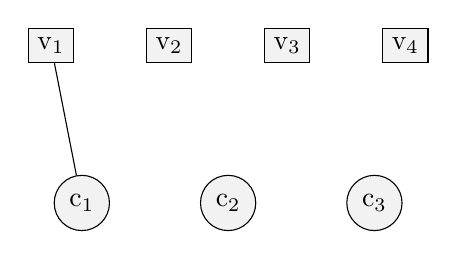
\begin{tikzpicture}
    % \draw (-5,-2) grid (5,2);

    \def\dist{1.5cm}
  \tikzset{node common/.style={draw, anchor=center, minimum size=0.2cm,fill=gray!10}}
  \tikzset{variable node/.style={node common}}
  \tikzset{check node/.style={node common, circle}}

  \coordinate (origin) at (0, 0);

  \path (origin) -- ++(-1.5*\dist, 0) coordinate (upline);


  % \coordinate (upline) at (0,0);
  \node[variable node] (v1) at ($(origin)+(-1.5*\dist,0)$) {$\mathrm{v}_1$};
  \node[variable node] (v2) at ($(origin)+(-0.5*\dist,0)$) {$\mathrm{v}_2$};
  \node[variable node] (v3) at ($(origin)+(0.5*\dist,0)$) {$\mathrm{v}_3$};
  \node[variable node] (v4) at ($(origin)+(1.5*\dist,0)$) {$\mathrm{v}_4$};
  %
  %
  % \coordinate (downline) at (2,2);
  \node[check node] (c2) at ($(origin)+(0, -2)$) {$\mathrm{c}_2$} ;
  \node[left=\dist of c2, check node] (c1) {$\mathrm{c}_1$};
  \node[right=\dist of c2, check node] (c3) {$\mathrm{c}_3$};
  %
  %
  \draw (v1) to (c1);
  %
  % % \draw (0,0) -- (1,1) -- ++(1,-1) coordinate (a)  -- +(1,2);

  % \draw[fill=red] (origin) circle (2pt);
  % \draw[fill=blue] (upline) circle (2pt);

  % \draw[blue]  (a) -- ++(0,-1);
\end{tikzpicture}

\end{document}
